\documentclass[aspectratio=169]{beamer}
%
%=====================================================================
%
\usetheme{Madrid}
\usecolortheme{default}
%
%=====================================================================
%
% Packages
\usepackage[utf8]{inputenc}
\usepackage{graphicx}
\usepackage{amsmath}
\usepackage{amssymb}
\usepackage{booktabs}
\usepackage{multicol}
%
%=====================================================================
%
% Title page information
\title{Text Based Analysis of Emerging Risks}
\subtitle{From Cyber Risk to Multi-Risk Classification}
\author{Giovanni Della Lunga}
\institute{University of Bologna}
\date{\today}
%
%=====================================================================
%
\begin{document}

\frame{\titlepage}
%
%..................................................................
%
\begin{frame}{Overview}
\begin{itemize}
    \item \textbf{Current Focus}: Text-based measures of cyber risk using news attention indices
    \item \textbf{Methodology}: Natural language processing applied to financial risk assessment
    \item \textbf{Future Development}: Extension to multi-label classification of emerging risks
    \item \textbf{Key Innovation}: From single-risk attention indices to comprehensive risk taxonomy
\end{itemize}

\vspace{0.5cm}
\begin{block}{Research Question}
Can text-based analysis effectively identify and classify multiple emerging risks (climate, cyber, geopolitical) in corporate disclosures and news media?
\end{block}
\vspace{0.2cm}
\small
U. Cherubini (University of Bologna) - G. Della Lunga (University of Bologna)- G. Figà Talamanca (University of Perugia) - B. Guardabascio (University of Perugia) \textit{Text-Based Measures of Cyber Risk, The Economic Impact of Cyber Risk News}. Work in progress.

\end{frame}
%
%..................................................................
%
\begin{frame}{Current Methodology: Cyber News Attention Index (CNAI)}
\begin{columns}
\begin{column}{0.6\textwidth}
\textbf{Data Sources:}
\begin{itemize}
    \item 5 major newspapers (2014-2023)
    \item Financial Times, LA Times, NY Times, USA Today, WSJ
    \item 10-year temporal horizon
\end{itemize}

\textbf{Processing Pipeline:}
\begin{enumerate}
    \item Text preprocessing (tokenization, stopword removal)
    \item Keyword-based scoring (0-10 scale)
    \item Daily/weekly/monthly aggregation
    \item Validation with Google Trends
\end{enumerate}
\end{column}
\begin{column}{0.4\textwidth}
\begin{block}{Keywords Examples}
\begin{itemize}
    \item malware
    \item phishing
    \item data breach
    \item ransomware
    \item unauthorized access
\end{itemize}
\end{block}
\end{column}
\end{columns}
\end{frame}
%
%..................................................................
%
\begin{frame}{Current Methodology: Cyber News Attention Index (CNAI)}
\begin{center}
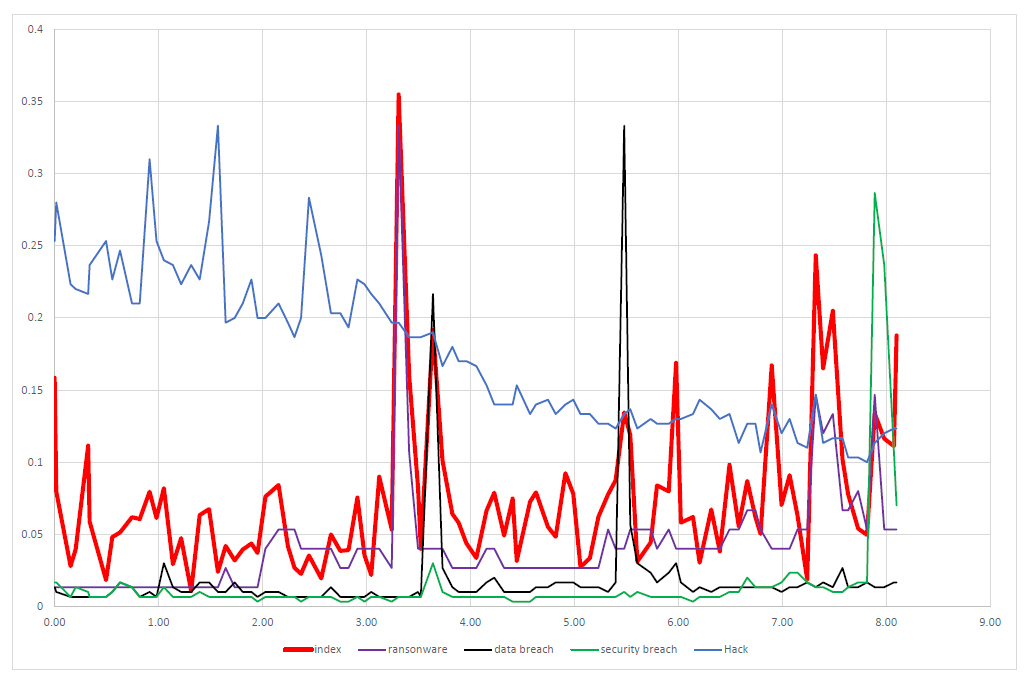
\includegraphics[scale=.375]{index.PNG} 
\end{center}
\end{frame}
%
%..................................................................
%
\begin{frame}{CNAI Validation: Major Cyber Events Detected}
\begin{table}[h]
\centering
\small
\begin{tabular}{ll}
\toprule
\textbf{Date} & \textbf{Event} \\
\midrule
May 2017 & WannaCry Ransomware (200K+ computers) \\
Sep 2017 & Equifax Breach (143M people affected) \\
Dec 2020 & SolarWinds Hack (US gov agencies) \\
May 2021 & Colonial Pipeline Ransomware \\
Dec 2021 & Log4j Vulnerability \\
\bottomrule
\end{tabular}
\end{table}

\vspace{0.3cm}
\begin{itemize}
    \item \textbf{18 "months of attention"} identified (threshold-based)
    \item Strong correlation with Google Trends data
    \item External validation through ChatGPT event identification
\end{itemize}
\end{frame}
%
%..................................................................
%
\begin{frame}{Empirical Analysis: Market Impact Assessment}
\begin{columns}
\begin{column}{0.5\textwidth}
\textbf{Mimicking Portfolio Approach:}
$$\Delta CNAI_t = \alpha + \beta Z_t^{Cyb} + \gamma' Z_t + \omega_t$$

Where $Z^{Cyb} \equiv R'(I_A - I_{NA})$
\begin{itemize}
    \item Long-short portfolio
    \item Attacked vs. non-attacked firms
    \item Controls: market indices, size, value factors
\end{itemize}
\end{column}
\begin{column}{0.5\textwidth}
\textbf{Local Projection Analysis:}
$$R_{i,t+k} = \alpha_k + \beta_k \Delta CNAI_t + \gamma_k' Z_t + \epsilon_{t+k}$$

\begin{itemize}
    \item Impulse response functions
    \item Sector-level analysis (GICS)
    \item Multi-horizon effects ($k = 1, ..., n$)
\end{itemize}
\end{column}
\end{columns}
\end{frame}
%
%..................................................................
%
\begin{frame}{Firm-Based Data}
\begin{itemize}
\item In the United States, publicly traded companies are required to periodically submit documents to the Securities and Exchange Commission (SEC) to ensure transparency and investor protection.
\item The main disclosure forms include:
\begin{itemize}
\item Form 10-K (annual report)
\item Form 10-Q (quarterly report)
\item Form 8-K (current report for material events)
\end{itemize}
\end{itemize}
\end{frame}
%
%..................................................................
%
\begin{frame}{Form 10-K}
\begin{itemize}
\item \textbf{Definition:} Form 10-K is the annual report that publicly traded companies must submit to the SEC, providing a comprehensive overview of their financial performance.
\item \textbf{Content:}
\begin{itemize}
\item Company history and organizational structure.
\item Audited financial statements.
\item Analysis of economic-financial results.
\item Description of business strategy.
\item Discussion of risk factors.
\item Governance information.
\end{itemize}
\item \textbf{Filing deadlines:}
\begin{itemize}
\item Large Accelerated Filers (market capitalization $\ge$ 700 million USD): within 60 days of fiscal year end.
\item Accelerated Filers (market capitalization between 75 and 700 million USD): within 75 days.
\item Non-Accelerated Filers (market capitalization < 75 million USD): within 90 days.
\end{itemize}
\end{itemize}
\end{frame}
%
%..................................................................
%
\begin{frame}{Form 10-K}
\begin{center}
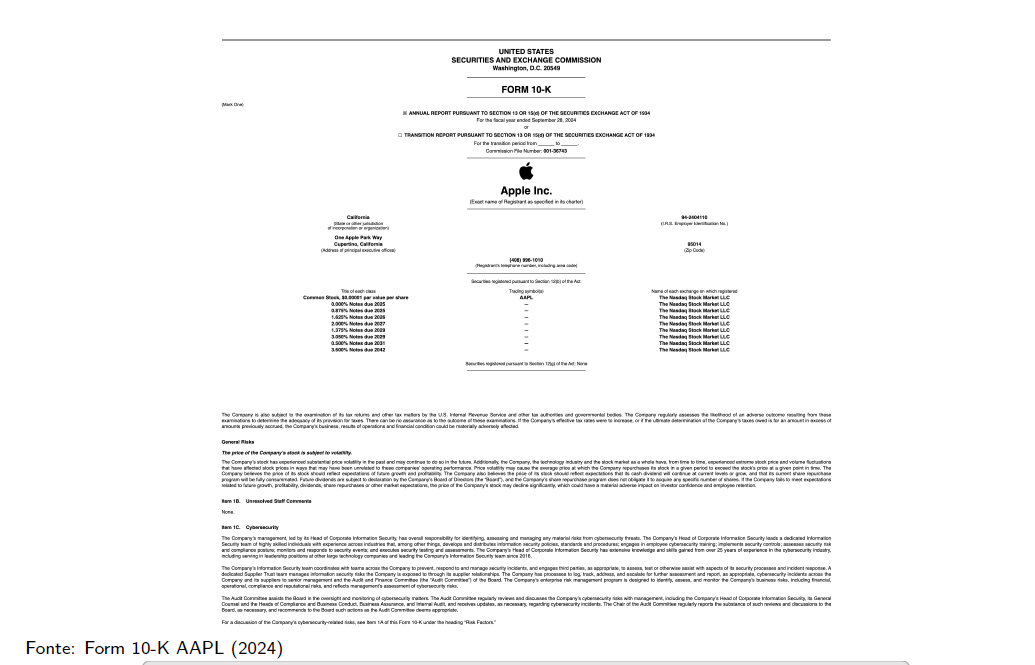
\includegraphics[scale=.4]{10-K.PNG} 
\end{center}
\end{frame}
%
%..................................................................
%
\begin{frame}{Form 8-K}
\begin{itemize}
\item \textbf{Definition:} Form 8-K is a current report used to communicate material corporate events that occur between periodic filings.
\item \textbf{Examples of events to report:}
\begin{itemize}
\item Changes in corporate leadership.
\item Significant acquisitions or divestitures.
\item Bankruptcies.
\item Material cybersecurity incidents.
\end{itemize}
\item \textbf{Filing timeline:} Companies must file Form 8-K within 4 business days of the event (with possible extension up to 60 days).
\end{itemize}
\end{frame}
%
%..................................................................
%
\begin{frame}{Form 8-K}
\begin{center}
\includegraphics[scale=.4]{8-K.PNG} 
\end{center}
\end{frame}
%
%..................................................................
%
\begin{frame}{Data Integration: SEC 8-K Forms Analysis}
\textbf{Regulatory Framework (Post-2023):}
\begin{itemize}
    \item Mandatory cyber incident disclosure (Item 1.05)
    \item 4-day filing requirement
    \item Material cybersecurity events
\end{itemize}

\textbf{Processing Pipeline:}
\begin{enumerate}
    \item Python + edgartools library for EDGAR access
    \item Keyword-based filtering (20\% threshold)
    \item GPT-4 classification of attack types
    \item Entity extraction (organizations, individuals, locations)
    \item PostgreSQL storage for structured analysis
\end{enumerate}

\textbf{Limitation:} Disclosure mandatory only from 2023 → retrospective vulnerability assumption
\end{frame}
%
%..................................................................
%
\begin{frame}{BERT for Document Classification}
\begin{itemize}
\item \textbf{What is BERT?}
\begin{itemize}
\item Bidirectional Encoder Representations from Transformers (Google, 2018)
\item Pre-trained language model that understands context from both directions
\item Captures deep semantic meaning and relationships in text
\end{itemize}

\item \textbf{How BERT Works for Classification:}
\begin{itemize}
\item \textbf{Input:} Document text is tokenized and fed to BERT with special [CLS] token
\item \textbf{Processing:} BERT generates contextualized embeddings for each token
\item \textbf{Classification:} [CLS] token representation is used for final classification layer
\item \textbf{Fine-tuning:} Model is adapted to specific classification tasks with labeled data
\end{itemize}
\end{itemize}
\end{frame}
%
%..................................................................
%
\begin{frame}{BERT for Document Classification}
\begin{itemize}

\item \textbf{Applications for Document Classification:}
\begin{itemize}
\item Sentiment analysis (positive/negative/neutral)
\item Topic classification (finance, technology, healthcare, etc.)
\item Document type identification (reports, emails, contracts)
\item Risk assessment and compliance categorization
\end{itemize}

\item \textbf{Advantages:}
\begin{itemize}
\item High accuracy due to contextual understanding
\item Transfer learning capabilities from pre-trained models
\item Handles complex linguistic patterns and domain-specific terminology
\end{itemize}
\end{itemize}
\end{frame}
%
%..................................................................
%
\begin{frame}{Future Development: Multi-Risk BERT Classification}
\begin{block}{Objective}
Extend methodology to classify firms into multiple emerging risk categories using 10-K and 8-K disclosures
\end{block}

\textbf{Target Risk Categories:}
\begin{multicols}{2}
\begin{itemize}
    \item Climate Physical Risk
    \item Climate Transition Risk
    \item Cybersecurity Risk
    \item Geopolitical Risk
    \item Supply Chain Risk
    \item Regulatory Risk
    \item Pandemic Risk
\end{itemize}
\end{multicols}

\textbf{Data Source:} Item 1A. Risk Factors section of 10-K filings
\end{frame}
%
%..................................................................
%
\begin{frame}{Advanced Methodological Approaches}
\begin{columns}
\begin{column}{0.5\textwidth}
\textbf{1. Weak Supervision (Snorkel):}
\begin{itemize}
    \item Labeling functions for scalability
    \item Keyword-based heuristics
    \item Probabilistic label generation
    \item Reduced manual annotation effort
\end{itemize}

\textbf{2. Zero-Shot Classification:}
\begin{itemize}
    \item Natural Language Inference models
    \item BART-large-mnli, RoBERTa-base
    \item No training data required
    \item Flexible for emerging risk types
\end{itemize}
\end{column}
\begin{column}{0.5\textwidth}
\textbf{3. Hybrid Strategy:}
\begin{enumerate}
    \item Zero-shot for initial classification
    \item Generate pseudo-labels
    \item Train Snorkel labeling functions
    \item Fine-tune BERT on combined data
\end{enumerate}

\begin{block}{Advantage}
Combines rapid prototyping with scalable, structured control over labeling process
\end{block}
\end{column}
\end{columns}
\end{frame}
%
%..................................................................
%
\begin{frame}
\frametitle{What is Snorkel and Weak Labeling?}

\textbf{The Problem:}
\begin{itemize}
\item Manual data labeling is \textbf{expensive} and \textbf{time-consuming}
\item Need thousands of labeled examples to train ML models
\item Expert annotators are costly and may disagree
\end{itemize}

\vspace{0.5cm}

\textbf{Snorkel's Solution: Weak Supervision}
\begin{enumerate}
\item \textbf{Labeling Functions}: Simple rules that assign labels
\begin{itemize}
\item Example: ``If text contains `data breach' $\rightarrow$ Cyber Risk''
\item Example: ``If text mentions `carbon emissions' $\rightarrow$ Climate Risk''
\end{itemize}

\item \textbf{Multiple Noisy Sources}:
\begin{itemize}
\item Keyword matching
\item Regular expressions
\item External databases
\item Existing models
\end{itemize}

\item \textbf{Statistical Combination}: Snorkel learns source reliability and combines them
\end{enumerate}

\textbf{Key Advantage}: Label thousands of documents automatically with reasonable accuracy

\end{frame}
%
%..................................................................
%
\begin{frame}
\frametitle{What is Zero-Shot Learning?}

\textbf{Traditional Machine Learning:}
\begin{center}
Training Data $\rightarrow$ Train Model $\rightarrow$ Predict on New Data
\end{center}
\textit{Need labeled examples for each category}

\vspace{0.5cm}

\textbf{Zero-Shot Learning:}
\begin{center}
Pre-trained Model + Task Description $\rightarrow$ Direct Prediction
\end{center}
\textit{No training examples needed!}

\vspace{0.5cm}

\textbf{How it Works:}
\begin{itemize}
\item Use large language models (BART, RoBERTa) trained on massive text
\item Provide natural language descriptions of categories:
\begin{itemize}
\item ``This text discusses cybersecurity threats and data breaches''
\item ``This text covers climate change and environmental risks''
\end{itemize}
\item Model uses learned language understanding to classify
\end{itemize}

\vspace{0.3cm}

\textbf{Advantages:}
\begin{itemize}
\item Rapid prototyping for new risk categories
\item No need for labeled training data
\item Flexible adaptation to emerging risks
\end{itemize}

\end{frame}
%
%..................................................................
%
\begin{frame}
\frametitle{Combining Snorkel and Zero-Shot Learning}

\textbf{Hybrid Strategy - Best of Both Worlds:}

\vspace{0.3cm}

\begin{enumerate}
\item \textbf{Start with Zero-Shot}
\begin{itemize}
\item Quickly classify large dataset
\item No manual labeling required
\item Generate initial pseudo-labels
\end{itemize}

\vspace{0.2cm}

\item \textbf{Create Snorkel Labeling Functions}
\begin{itemize}
\item Use zero-shot results to identify patterns
\item Write keyword-based rules
\item Add domain expertise through heuristics
\end{itemize}

\vspace{0.2cm}

\item \textbf{Combine and Refine}
\begin{itemize}
\item Snorkel weighs zero-shot + rule-based labels
\item Statistical model resolves conflicts
\item Produces higher-quality training data
\end{itemize}

\end{enumerate}
\end{frame}
%
%..................................................................
%
\begin{frame}{Conclusion}
\textbf{Current Achievements:}
\begin{itemize}
    \item Successful CNAI development with strong external validation
    \item Integration of news-based and regulatory disclosure data
    \item Theoretical framework connecting text measures to asset pricing
\end{itemize}

\textbf{Next Steps:}
\begin{itemize}
    \item Scale from single-risk (cyber) to multi-risk classification
    \item Implement BERT-based multi-label approach with weak supervision
    \item Develop comprehensive emerging risk taxonomy
    \item Create tradable risk indices for portfolio applications
\end{itemize}

\vspace{0.5cm}
\begin{center}
\textbf{Thank you for your attention!}
\end{center}
\end{frame}
%
%=====================================================================
%
\end{document}